\documentclass[10pt,journal,letterpaper]{IEEEtran}


\usepackage[utf8]{inputenc}
\usepackage[T1]{fontenc}
\usepackage{tgtermes}


\usepackage{microtype}
\frenchspacing


\usepackage{amsmath, amssymb, amsthm}


\usepackage{graphicx}
\usepackage{array}
\usepackage{booktabs}


\usepackage{cite}
\usepackage{xurl}
\usepackage[colorlinks=true,
            linkcolor=blue,
            filecolor=magenta,
            urlcolor=cyan,
            citecolor=blue]{hyperref}


\usepackage{placeins}


\newtheorem{theorem}{Theorem}
\newtheorem{definition}{Definition}
\newtheorem{lemma}{Lemma}
\newtheorem{remark}{Remark}
\renewcommand{\qedsymbol}{$\blacksquare$}


\title{Voronoi-Based Activation Functions and Inertial Energy for Complex-Valued Hopfield Networks}

\author{
Fidelis~Zanetti~de~Castro\textsuperscript{*},
Marcos~Eduardo~Valle\textsuperscript{\dag},
João~P.~Papa\textsuperscript{\ddag},
and~Rodolfo~Anibal~Lobo\textsuperscript{\S}
\thanks{\textsuperscript{*}F.~Z.~Castro is with the Federal Institute of Education, 
        Science and Technology of Esp\'irito Santo at Serra, 
        Serra, ES, Brazil. (e-mail: fidelis@ifes.edu.br).}
\thanks{\textsuperscript{\dag}M.~E.~Valle is with the Department of Applied Mathematics, 
        Universidade Estadual de Campinas, 
        Campinas, SP, Brazil. (e-mail: valle@ime.unicamp.br).}
\thanks{\textsuperscript{\ddag}J.~P.~Papa is with the Department of Computing, 
        S\~ao Paulo State University, Bauru, SP, Brazil. (e-mail: joao.papa@unesp.br).}
\thanks{\textsuperscript{\S}R.~A.~Lobo is with Globant Company, 
        Santiago, Chile. (e-mail: rodolfo.\allowbreak{}lobo@\allowbreak{}globant.com).}
}

\begin{document}
% Keep natural paragraph/display spacing instead of stretching short columns
% around wide figures and tables to force an identical bottom baseline.
\raggedbottom

\maketitle

\begin{abstract}
Complex-valued Hopfield neural networks (CV-HNNs) usually rely on phase-only or constant-modulus alphabets, for which the classical inner-product update is naturally aligned with the usual Hopfield energy. This paper considers finite alphabets that encode both phase and magnitude. We show that, on multi-amplitude constellations, the classical update may exhibit a magnitude saturation bias: outer symbols can be selected even when inner symbols are closer to the local field in the Euclidean geometry of the complex plane. To overcome this limitation, we introduce an alphabet-dependent Voronoi activation that projects each local field onto the nearest symbol of the prescribed constellation, covering Phase-Shift Keying (PSK), Quadrature Amplitude Modulation (QAM), polar, hexagonal, and irregular alphabets in a common framework. We also derive the corresponding inertial energy and prove finite convergence of the asynchronous dynamics under Hermitian weights with nonnegative diagonal entries and conservative deterministic tie handling. Computational experiments confirm the predicted radial behavior, illustrate the effect in hue-saturation-value (HSV)-encoded associative recall, and show that exact implementations based on $k$-dimensional tree (KD-tree) search or structured quantizers can substantially reduce the cost of evaluating the proposed activation.
\end{abstract}

\begin{IEEEkeywords}
Complex-valued Hopfield networks, magnitude saturation bias, Voronoi projection, 
inertial energy, multi-amplitude alphabets.
\end{IEEEkeywords}

\section{Introduction}

\IEEEPARstart{T}{he} associative-memory paradigm introduced by Hopfield in 1982~\cite{hopfield1982} and grounded in the absolute stability theorems of Cohen and Grossberg~\cite{cohen1983} has strongly influenced the development of recurrent neural networks. By associating memories with attractors of a recurrent dynamical system and by providing an energy function that decreases under asynchronous updates, Hopfield-type models offer a rigorous mechanism for content-addressable memory, error correction, and pattern completion. Although the original model is binary, many applications require neural states with richer representational structure.

CV-HNNs extend the associative-memory framework by allowing neural states, synaptic weights, and local fields to take values in the complex plane. Complex representations retain the phase and amplitude information of wave-based signals~\cite{hirose2009merits}. Applications include interferometric radar image processing~\cite{hirose2001radar} and coherent optical computing~\cite{hirose1994optical}; complex constellations also provide a standard representation of communication signals~\cite{proakis2008}. In associative memory, multivalued neurons have been used for gray-scale images~\cite{aizenberg1992}, and nonlinear multilevel complex activations have been studied for gray-level image reconstruction~\cite{tanaka2009}. A broader account of multivalued complex neurons is given in~\cite{aizenberg2011}. Early discrete-time complex-valued associative memories followed a phasor or multistate route: the state of each neuron is selected from a finite set of complex numbers on the unit circle. Noest's phasor network~\cite{noest1988}, the multistate associative memory of Jankowski \textit{et al.}~\cite{jankowski1996}, complex bidirectional associative memories~\cite{lee1999}, and design methods for multistate CV-HNNs~\cite{muezzinoglu2003} are representative examples of the phasor approach. In these models, the activation function normalizes or quantizes the phase of the local field, so information is encoded essentially in the angular coordinate.

A second route is based on split or componentwise activation functions. Instead of quantizing only the phase, a split activation applies a real-valued nonlinearity separately to the real and imaginary parts of the local field. For example, the split-sign function maps a complex number $a+b\mathbf{i}$ to $\operatorname{sign}_{\mathbb{R}}(a)+\operatorname{sign}_{\mathbb{R}}(b)\mathbf{i}$, producing the Cartesian alphabet $\{a+b\mathbf{i}:a,b\in\{-1,1\}\}$. The split-sign construction is a direct complex analogue of the bipolar Hopfield neuron. Related state representations and activation rules have been studied in quaternionic associative memories~\cite{isokawa2008associative,valle2016quaternionic}, commutative-quaternion networks~\cite{isokawa2010commutative,isokawa2011stabilitycommutative}, octonion networks~\cite{castro2018octonionic,kuroe2016octonion}, and Clifford recurrent networks~\cite{kuroe2011clifford}. Split-quaternion models have their own fixed-point analysis~\cite{kobayashi2017splitquaternion} and twin-multistate construction~\cite{kobayashi2020splittwin}. A general framework for discrete-time hypercomplex Hopfield networks is developed in~\cite{castro2020broad}; hypercomplex recurrent correlation memories provide a related extension~\cite{valle2021hypercomplexrcnn}. The split-sign alphabet still has constant modulus, but more general componentwise multilevel or ceiling-type activations lead naturally to finite alphabets with nonconstant magnitudes.

Substantial progress has also been made on the stability, fixed points, recall rules, and noise tolerance of complex and hypercomplex Hopfield memories~\cite{castro2018stability}. In particular, Kobayashi's work has shown that the behavior of these models is highly sensitive to the interaction between the state alphabet, the activation rule, the connection structure, and the update mode. His studies include hybrid quaternionic networks~\cite{kobayashi2014hybrid} and multistate vector-product networks~\cite{kobayashi2017vectorproduct}. For rotor networks, they address complex-number decompositions~\cite{kobayashi2017decomposition}, synchronous stability~\cite{kobayashi2018rotorstability}, and diagonal connections~\cite{kobayashi2020diagonalrotor}. Hyperbolic models have been investigated with directional multistate activations~\cite{kobayashi2018hyperbolic}, synchronous updates~\cite{kobayashi2020hyperbolicsync}, and hybrid updates~\cite{kobayashi2021hyperbolichybrid}. Other contributions establish stability conditions for bicomplex networks~\cite{kobayashi2021bicomplexstability}, introduce twin-hyperbolic bicomplex networks~\cite{kobayashi2021bicomplextwin}, develop noise-robust projection rules for rotor and matrix-valued networks~\cite{kobayashi2022noise}, and formulate algebraic Hopfield networks~\cite{kobayashi2025algebraic}. Symmetric CV-HNNs were proposed to reduce the rotational invariance that degrades noise tolerance in standard complex-valued memories~\cite{kobayashi2017symmetric}, and their fixed points were subsequently analyzed in detail~\cite{kobayashi2018fixed}. Generalized projection rules improve complex associative memory~\cite{lee2001}, while fast-recall strategies address retrieval in networks using projection rules~\cite{kobayashi2017fastrecall}. Further variants, including two-level CV-HNNs~\cite{kobayashi2021twolevel}, real-weight complex-valued networks in synchronous mode~\cite{kobayashi2021realweights}, and hybrid complex-valued associative memories~\cite{kobayashi2025hybrid}, reinforce the same lesson: robust multistate associative memory depends not only on the storage rule, but also on the geometry induced by the activation and by the selected state space.

Synaptic asymmetry provides another direction of investigation.
Garimella, Swamy, and Valle~\cite{garimella2026orientation} formalize orientation
selectivity in asymmetric discrete-time Hopfield neural networks with bipolar states: interpreting
states as row or column vectors produces distinct left- and right-side
dynamics. They analyze rank-one asymmetric weights and propose a recording
rule based on convex optimization for associative memory. The present
analysis retains Hermitian weights and asks a different question: how does
the geometry of a finite, multi-amplitude alphabet affect local decisions
and their associated energy? Accordingly, our convergence theorem concerns
the stated Hermitian setting and does not assert convergence for general
asymmetric networks.

Most of these developments either preserve a constant-modulus state alphabet or address other structural aspects of complex and hypercomplex Hopfield dynamics. This convention is mathematically convenient. When all candidate states have the same modulus, the classical inner-product decision rule does not have to trade phase alignment against candidate magnitude. As a result, the usual Hopfield energy remains naturally aligned with the asynchronous local update, and convergence proofs can be obtained under standard assumptions on the synaptic matrix. However, the constant-modulus restriction also removes one of the two degrees of freedom of a complex number. A full-amplitude constellation, such as QAM, uses both phase and magnitude to encode information~\cite{proakis2008}. Recent phase-and-magnitude-quantized CV-HNNs based on ceiling-type activations explicitly move in this direction~\cite{garimella2025}. These works motivate the relevance of amplitude-bearing state spaces; the present contribution is to isolate the geometric consequence of using the classical inner-product decision on such alphabets and to supply a Lyapunov structure for the corresponding Voronoi-corrected dynamics.

Allowing multiple amplitudes raises a basic geometric question that is not isolated by phase-only, split-sign, or constant-modulus formulations: what happens to the classical Hopfield decision rule when the finite state alphabet contains symbols with different moduli? We show that the usual inner-product update introduces a structural magnitude saturation bias in such alphabets. Because the classical local score scales linearly with the modulus of the candidate state, high-modulus symbols may be selected even when lower-modulus symbols are geometrically closer to the local field. Thus, the problem is not a lack of energy descent in the classical sense; rather, it is a geometric mismatch between an unregularized inner-product score and a multi-amplitude constellation.

To address this mismatch, we propose a constellation-dependent activation
function defined by Euclidean, or Voronoi, projection onto an arbitrary finite
alphabet $\mathcal{S}\subset\mathbb{C}$, mapping each local field
to the nearest complex state and thereby generalizing phase quantization and
componentwise quantization without committing to a particular coordinate
system. Algebraically, the Voronoi decision is equivalent to maximizing the
classical local score with an additional quadratic penalty on the candidate
magnitude. This penalty leads to an inertial Lyapunov functional associated
with $\boldsymbol{W}-\boldsymbol{I}$ rather than $\boldsymbol{W}$ alone.

A related use of Voronoi geometry appears in the modern Hopfield network
(MHN) literature. Hashimoto \textit{et al.}~\cite{hashimoto2026voronoi}
propose a distance-based energy built from a softmin-weighted average of
squared distances to stored real-valued patterns. Their construction organizes
retrieval in the full pattern space. Here, Voronoi projection instead acts
on each neuron's complex local field, with the finite alphabet symbols as
generators. The resulting asynchronous dynamics uses Hermitian synaptic
weights and the quadratic inertial energy derived below. This distinction
locates the present contribution at the level of the neuron activation and
its associated convergence guarantee.

Precisely, the main contributions of this work are the following. First, we
identify the magnitude saturation bias of the classical inner-product update
and relate it to the geometry of finite multi-amplitude alphabets. Second, we
introduce the alphabet-dependent Voronoi activation
$\mathcal{D}_{\mathcal{S}}$, which replaces the fixed complex signum rule by a
projection explicitly determined by the chosen state alphabet. Third, we derive
the corresponding inertial energy functional and prove finite convergence of
the asynchronous dynamics under Hermitian weights with nonnegative diagonal
entries, a fair update schedule, and conservative deterministic tie handling.
Accordingly, the paper does not merely propose a new quantizer; it supplies the
Lyapunov structure required to analyze the resulting Hopfield dynamics.

The remainder of this paper is organized as follows. Section~\ref{sec:prelim} revisits the geometric foundations of complex numbers and finite state alphabets. Section~\ref{sec:bias} formalizes the magnitude saturation bias of the classical update. Section~\ref{sec:voronoi} introduces the alphabet-dependent Voronoi activation and derives the associated inertial energy. Section~\ref{sec:experiments} presents computational experiments on geometric diagnostics, HSV associative-memory retrieval, and activation cost. Section~\ref{sec:conclusion} concludes with implications and directions for future work.

\section{Preliminaries and Geometric Foundations}
\label{sec:prelim}

\subsection{Complex Numbers: Algebraic and Polar Representations}

The complex field $\mathbb{C}$ is the natural ambient space for signals carrying 
both amplitude and phase. We briefly recall the standard representations used 
throughout the paper.

A complex number $z \in \mathbb{C}$ can be written in \textbf{algebraic form} as
\begin{equation}
    z = x + y\mathbf{i},
\end{equation}
where $x, y \in \mathbb{R}$ and $\mathbf{i}$ denotes the imaginary unit 
($\mathbf{i}^2 = -1$). The real and imaginary parts of $z$ are, respectively,
\begin{equation}
    \operatorname{Re}(z) = x, \qquad \operatorname{Im}(z) = y.
\end{equation}
The \textbf{modulus} (or absolute value) of $z$ is the non-negative real number
\begin{equation}
    |z| = \sqrt{x^2 + y^2}.
\end{equation}
Every non-zero $z$ admits a \textbf{polar form}
\begin{equation}
    z = r e^{\mathbf{i}\theta}, \qquad r = |z|, \quad \theta = \arg(z),
\end{equation}
where the \textbf{phase} (or argument) $\theta$ is defined up to an integer multiple 
of $2\pi$; when a principal value is needed, we take $\arg(z) \in (-\pi,\pi]$. 
The algebraic and polar representations are linked by Euler's formula
$e^{\mathbf{i}\theta} = \cos\theta + \sin\theta\,\mathbf{i}$.

The mapping
\begin{equation}
    z = x + y\mathbf{i} \;\longleftrightarrow\; (x,y) \in \mathbb{R}^2
\end{equation}
is an $\mathbb{R}$-linear isometry, since $|z| = \|(x,y)\|$ and addition in 
$\mathbb{C}$ naturally corresponds to vector addition in $\mathbb{R}^2$. This isomorphism 
allows us to freely translate geometric concepts between $\mathbb{C}$ and the 
Euclidean plane. In particular, the Euclidean distance between two points 
$z,w\in\mathbb{C}$ is $|z-w|$, and the standard inner product in $\mathbb{R}^2$ 
is recovered by $\langle z, w \rangle = \operatorname{Re}(\overline{z} w)$.

\paragraph*{Notation}
Scalars in $\mathbb{C}$ are denoted by lower-case letters, whereas vectors and
matrices are denoted by boldface symbols. The complex conjugate of a scalar
$z$ is written as $\overline{z}$. For vectors and matrices, the superscript
$*$ denotes conjugate transpose; for example, $\boldsymbol{W}=\boldsymbol{W}^*$
means that $\boldsymbol{W}$ is Hermitian. Thus, scalar conjugation is always
written with an overbar, while $*$ is reserved for vector and matrix
transposition with conjugation.

\subsection{Complex State Alphabets, Voronoi Cells, and Maximum Modulus}

We now formalize the geometric structures that govern discrete complex-valued neural networks~\cite{aurenhammer2013voronoi}.

\begin{definition}[Complex state alphabet]
A \textbf{complex state alphabet} is a nonempty finite set
$\mathcal{S} \subset \mathbb{C}$. Each element $s\in\mathcal{S}$ represents a
possible state of a single neuron. The cardinality $M = |\mathcal{S}|$ denotes the
alphabet size, or number of symbols.
\end{definition}

\begin{definition}[Maximum modulus and saturation boundary]
\label{def:maximum_modulus}
The \textbf{maximum modulus} of a state alphabet is
\begin{equation}
    R_{\max} = \max_{s \in \mathcal{S}} |s|.
\end{equation}
The set
\begin{equation}
    \partial_{\max}\mathcal{S}
    = \bigl\{s\in\mathcal{S}: |s|=R_{\max}\bigr\}
\end{equation}
is called the \textbf{amplitude saturation boundary} of $\mathcal{S}$.
\end{definition}

The amplitude saturation boundary will be central in Section~\ref{sec:bias}. In
classical inner-product dynamics, the local score scales linearly with the
candidate modulus; hence, when $\mathcal{S}$ contains nonconstant moduli, the
update may favor outermost states even when inner states are geometrically closer
to the local field.

\begin{definition}[Voronoi cell and boundaries]
For a given set of complex states $\mathcal{S}$, the \textbf{Voronoi cell} (or Voronoi 
region) of a point $s \in \mathcal{S}$ is the set
\begin{equation}
    V(s) = \bigl\{ z \in \mathbb{C} : |z - s| \le |z - s'| 
           \;\text{for all}\; s' \in \mathcal{S} \bigr\}.
\end{equation}
The \textbf{Voronoi diagram} of $\mathcal{S}$ is the covering of the complex 
plane by the closed cells $\{V(s)\}_{s\in\mathcal{S}}$. The \textbf{Voronoi boundaries}
are the points with two or more nearest symbols in $\mathcal{S}$, defined by
the set $\bigcup_{s\neq s'} V(s)\cap V(s')$.
\end{definition}

The Voronoi cell $V(s)$ is a closed convex polygon (or polyhedral region) containing exactly those points of $\mathbb{C}$ whose distance to $s$ is no greater than their distance to any other state. Distinct cells can intersect on their boundaries; the deterministic tie rule below resolves these shared points.

Figure~\ref{fig:voronoi_generic} illustrates the cells and their boundaries
for a sparse alphabet, together with its maximum-modulus symbols.

In the interior of a Voronoi cell, the proposed alphabet-dependent activation $\mathcal{D}_{\mathcal{S}}$ selects its generator. On shared boundaries, the selection also depends on the current state and the tie rule. This partition serves as the geometric counterpart to the inertial penalty $-\tfrac12|s|^2$ derived in Theorem~\ref{thm:stability}: instead of solely maximizing the projection $\operatorname{Re}(\overline{s}v_k)$, the dynamics selects the Euclidean nearest neighbor, thereby suppressing the drift toward the amplitude saturation boundary.

\begin{figure}[htbp]
    \centering
    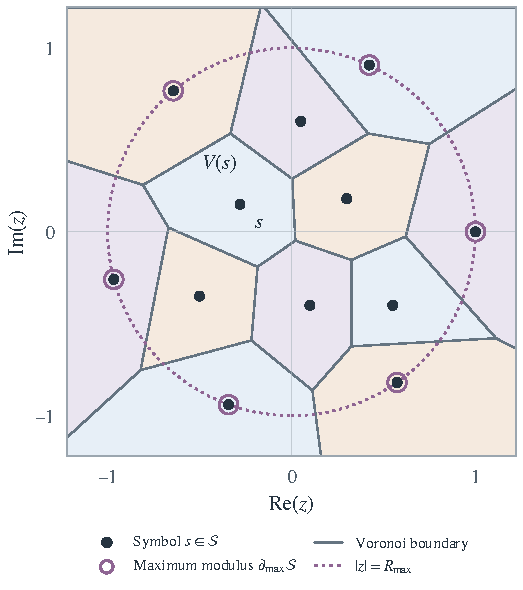
\includegraphics[width=1\linewidth]{Figures/generic_voronoi.pdf}
    \caption{A deliberately spaced, illustrative 12-symbol alphabet with $R_{\max}=1$. Filled dots denote symbols, hollow rings identify $\partial_{\max}\mathcal{S}$, and the dotted circle is $|z|=R_{\max}$. The labels $s$ and $V(s)$ identify one generator and its cell. Thin solid lines are Voronoi boundaries; pastel colors distinguish neighboring cells and have no quantitative meaning. All cells are clipped to the displayed window.}
    \label{fig:voronoi_generic}
\end{figure}

When the state alphabet contains points of varying moduli, the classical update
rule $\arg\max_{s\in\mathcal{S}} \operatorname{Re}(\overline{s}v_k)$ maximizes a 
linear functional that scales with $|s|$. Consequently, the system may favor 
states with larger magnitude even if their phase alignment is suboptimal. In typical 
multi-amplitude state alphabets (e.g., QAM), the points of maximum modulus coincide
with the outer ring or corner symbols. As such, the classical dynamics 
can move the network toward the amplitude saturation boundary, 
sacrificing the hierarchical resolution of inner states.

This paper focuses on four representative state geometries, each inducing a
characteristic Voronoi diagram (Fig.~\ref{fig:constellations}). These
definitions fix the notation used in the theoretical discussion and in all
computational experiments below; in particular, $M=|\mathcal{S}|$ denotes the
alphabet cardinality whenever the construction has exactly $M$ symbols.

\begin{definition}[PSK]
Uniform-magnitude symbols placed on the unit circle:
$\mathcal{S}_{PSK} = \bigl\{ e^{\mathbf{i} 2\pi k / M} \mid 
   k = 0, 1, \dots, M-1 \bigr\}$.
\end{definition}

All PSK symbols satisfy $|s|=1=R_{\max}$; hence, PSK has no amplitude hierarchy
and will serve as a constant-modulus control case.

\begin{definition}[QAM]
A Cartesian square lattice:
$\mathcal{S}_{QAM} = \bigl\{ (2m - 1 - \sqrt{M})d + 
   (2n - 1 - \sqrt{M})d\,\mathbf{i} \mid m,n = 1,\dots,\sqrt{M} \bigr\}$,
where $d>0$ is half the distance between adjacent states and $\sqrt{M}$ is assumed
to be an integer.
\end{definition}

For the corresponding infinite square lattice, interior Voronoi cells are
rectangles, and squares when the real and imaginary spacings coincide. For a
finite alphabet considered in the full complex plane, boundary cells are
generally unbounded; in plotted windows, they are displayed as clipped polygonal
regions. The four corner states have maximum modulus
$R_{\max}=\sqrt{2}(\sqrt{M}-1)d$.

\begin{definition}[Polar QAM / Concentric Rings]
A set combining discrete amplitudes and phases:
$\mathcal{S}_{Polar} = \bigl\{ r_m e^{\mathbf{i} \theta_n} \mid 
   r_m \in \mathcal{R},\; \theta_n \in \Theta \bigr\}$,
where $\mathcal{R} \subset \mathbb{R}_{>0}$ and $\Theta \subset [0,2\pi)$ are 
finite discrete sets.
\end{definition}

Under the Euclidean metric, the Voronoi regions induced by these ring-structured
points are convex polygonal cells, rather than circular annular sectors. The
states with maximum modulus lie on the outermost ring, establishing the
amplitude saturation boundary.

\begin{definition}[Eisenstein hexagonal lattice]
A packing-optimal configuration generated by the Eisenstein integers:
$\mathcal{S}_{Hex} = \bigl\{ a + b\omega \in \mathbb{C} \mid a,b \in \mathbb{Z},\;
   \omega = e^{\mathbf{i}2\pi/3} \bigr\} \cap \text{(finite window)}$.
\end{definition}

The Eisenstein lattice is the standard triangular/hexagonal lattice in the
complex plane and is closely related to optimal two-dimensional packing
geometries~\cite{conwaySloane1999}. Interior cells of the infinite lattice are
regular hexagons. For a finite window, boundary cells are unbounded in the full
plane or truncated in visualizations. The states of maximum modulus lie on the
boundary of the selected finite window and form the amplitude saturation
boundary.

These four geometries are deliberately chosen to isolate the role of amplitude variation:
\begin{itemize}
\item[(i)] PSK provides a control scenario where $|s|$ is constant, rendering the
classical rule immune to the magnitude bias;
\item[(ii)] Square QAM is the standard Cartesian multi-amplitude scheme in
telecommunications, featuring rectangular interior cells;
\item[(iii)] Polar QAM explicitly separates radial and angular degrees of freedom,
while still inducing Euclidean polygonal Voronoi cells;
\item[(iv)] The hexagonal lattice achieves optimal packing density in the
plane, demonstrating that the magnitude bias and its proposed correction hold for any finite set of complex states in $\mathbb{R}^2$, independent of the coordinate system.
\end{itemize}

\begin{definition}[Asynchronous update schedule and fairness]
An \textbf{asynchronous update schedule} is a sequence of neuron indices
$k_0,k_1,k_2,\ldots$ such that only coordinate $k_t$ is updated at time $t$. The
schedule is \textbf{fair} if no coordinate that remains eligible to change
is postponed indefinitely. For example, coordinates may be randomly selected
independently at each step with fixed strictly positive probabilities; the
resulting schedule is fair almost surely. A cyclic scan is also fair.
\label{def:fair_schedule}
\end{definition}

Tie handling will be deterministic throughout the paper. We fix, once and for
all, a total order $\preceq$ on the finite alphabet $\mathcal{S}$ and denote by
$\bigwedge_{\preceq} A$ the least element of any nonempty subset
$A\subseteq\mathcal{S}$. For example, one may order nonzero symbols
lexicographically in polar coordinates: if
$z_\ell=r_\ell e^{\mathbf{i}\theta_\ell}$, with
$r_\ell=|z_\ell|>0$ and
$\theta_\ell=\operatorname{Arg}(z_\ell)\in(-\pi,\pi]$, define
$z_1\preceq z_2$ whenever $r_1<r_2$, or $r_1=r_2$ and
$\theta_1\le\theta_2$. If $0\in\mathcal{S}$, it may be declared the least
symbol. The convergence result below only requires the order to be fixed; it
does not depend on this particular choice.

\begin{figure*}[!t]
    \centering
    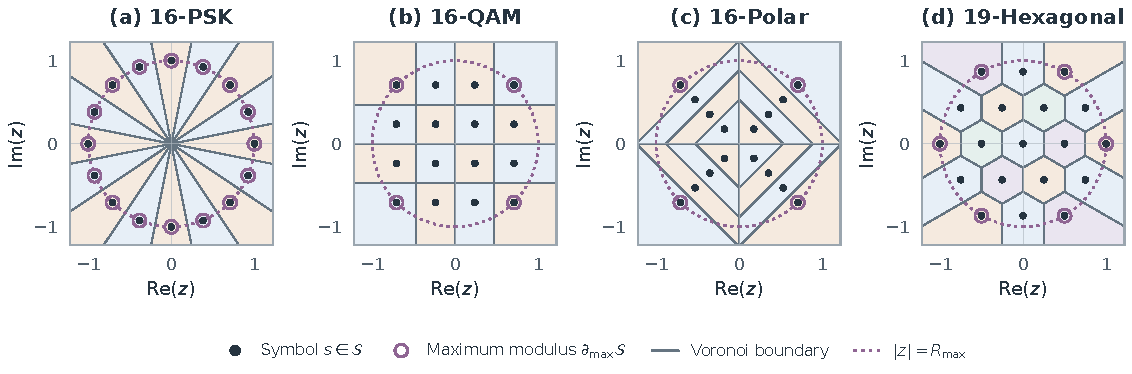
\includegraphics[width=\textwidth]{Figures/constellations.pdf}
    \caption{Four finite complex alphabets, normalized to $R_{\max}=1$, with exact planar Voronoi cells clipped to a common window. Filled dots denote symbols $s\in\mathcal{S}$; thin solid lines delimit the cells $V(s)$. Hollow rings mark $\partial_{\max}\mathcal{S}$, and the dotted circle is $|z|=R_{\max}$. All PSK symbols have maximum modulus. Pastel colors distinguish neighboring cells and do not encode a numerical quantity.}
    \label{fig:constellations}
\end{figure*}

\section{The Unregularized Magnitude Scaling and Magnitude Saturation Bias}
\label{sec:bias}

Consider a network of $N$ neurons with a column state vector $\boldsymbol{s}(t) \in \mathcal{S}^N$ and a Hermitian synaptic weight matrix $\boldsymbol{W}=\boldsymbol{W}^*$. The local activation field for neuron $k$ at time $t$ is expressed as
\begin{equation}
    v_k(t) = (\boldsymbol{W}\boldsymbol{s}(t))_k
           = \sum_{j=1}^N w_{kj}s_j(t)
           = \boldsymbol{w}_k^*\boldsymbol{s}(t),
\end{equation}
where $\boldsymbol{w}_k^*$ is the $k$-th row of $\boldsymbol{W}$. Every complex
decision functional considered below relies on the real inner product
$\operatorname{Re}(\overline{s}v)$.

The classical update rule operates by maximizing the real part of the complex
inner product. Let $\Psi_k(t)$ denote the set of maximizers of this classical
functional:
\begin{equation}
    \Psi_k(t) \triangleq \underset{s \in \mathcal{S}}{\arg\max} \operatorname{Re}(\overline{s} v_k(t)).
\end{equation}

To circumvent artificial transitions among tied maximizers, the classical update is defined piecewise. It preserves the current state if it is already a maximal candidate:
\begin{equation}
    s_k(t+1) = 
    \begin{cases} 
    s_k(t), & \text{if } s_k(t) \in \Psi_k(t) \\
    \bigwedge_{\preceq}\Psi_k(t), & \text{otherwise}.
    \end{cases}
\label{eq:classical_rule}
\end{equation}

To understand why this dynamic can degrade multi-amplitude structures despite possessing a deterministic tie-handling mechanism, we expand the inner product using Euler's formula. Let $s = |s|e^{\mathbf{i}\theta_s}$ 
and the local field $v_k = |v_k|e^{\mathbf{i}\theta_v}$. The maximization 
objective becomes:
\begin{equation}
    \operatorname{Re}(\overline{s} v_k) = |s| |v_k| \cos(\theta_s - \theta_v).
\label{eq:cosine_expansion}
\end{equation}

To quantify this unregularized scaling mechanism, we formalize a pairwise
magnitude-dominance condition.

\begin{lemma}[Pairwise Magnitude Dominance]
\label{lem:centrifugal_drift}
Let $v_k = |v_k|e^{\mathbf{i}\theta_v}$ be a non-zero local field. Suppose $\mathcal{S}$ contains an inner state $s_{\mathrm{in}} = r_{\mathrm{in}}e^{\mathbf{i}\theta_v}$ perfectly aligned with $v_k$, and an outer state $s_{\mathrm{out}} = r_{\mathrm{out}}e^{\mathbf{i}\theta_{\mathrm{out}}}$ such that $r_{\mathrm{out}} > r_{\mathrm{in}}>0$. Under the classical score $F(s)=\operatorname{Re}(\overline{s}v_k)$, the outer state $s_{\mathrm{out}}$ dominates the inner aligned state $s_{\mathrm{in}}$ pairwise if and only if
\begin{equation}
    \cos(\theta_{\mathrm{out}} - \theta_v) > \frac{r_{\mathrm{in}}}{r_{\mathrm{out}}}.
\end{equation}
Consequently, the classical update selects $s_{\mathrm{out}}$ whenever this
inequality holds and $s_{\mathrm{out}}$ also dominates every other candidate in
$\mathcal{S}$ under the same score.
\end{lemma}

\begin{proof}
The classical update seeks to maximize the functional $F(s) = \operatorname{Re}(\overline{s}v_k)$. For the perfectly aligned inner state, the objective yields $F(s_{\mathrm{in}}) = r_{\mathrm{in}}|v_k|\cos(0) = r_{\mathrm{in}}|v_k|$. For the misaligned outer state, $F(s_{\mathrm{out}}) = r_{\mathrm{out}}|v_k|\cos(\theta_{\mathrm{out}} - \theta_v)$. The outer state strictly dominates the inner state when $F(s_{\mathrm{out}}) > F(s_{\mathrm{in}})$. Since $|v_k| > 0$, dividing the inequality by $|v_k|$ directly gives $\cos(\theta_{\mathrm{out}} - \theta_v) > r_{\mathrm{in}} / r_{\mathrm{out}}$. The final claim follows from the global $\arg\max$ definition of $\Psi_k(t)$.
\end{proof}

This lemma shows, at the pairwise level, how a higher-magnitude state can
dominate an inner-radius state that is geometrically aligned with the local
field. For instance, in a normalized 16-QAM set, an inner state
($r \approx 0.316$) can lose pairwise to a saturated corner state
($r \approx 0.948$) even if the corner state deviates by up to
$\arccos(1/3) \approx 70.5^\circ$ from the true local-field phase.

We call this phenomenon the \textit{Magnitude Saturation Bias}. Because the
objective score scales linearly with $|s|$, the classical rule may sacrifice
Euclidean proximity to exploit the unregularized scaling of the cosine
expansion, thereby favoring states near the amplitude saturation boundary and
reducing the resolution carried by inner states.

\section{Alphabet-Dependent Voronoi Dynamics and Structural Inertia}
\label{sec:voronoi}

\subsection{Constellation-Dependent Voronoi Activation}

The first central contribution of this section is to replace the fixed
complex signum/projection rule by an activation determined explicitly by the
finite alphabet $\mathcal{S}$. The rule is a nearest-neighbor decision in the
Voronoi diagram of the constellation~\cite{aurenhammer2013voronoi}, and it is
related in spirit to projection-based recall strategies previously considered
for CV-HNNs~\cite{lee2001,kobayashi2017fastrecall}.
The difference here is that the Voronoi decision is used as the activation
itself for an arbitrary finite alphabet, and the associated energy is derived
below. For a local field $v\in\mathbb{C}$, let
$\Omega_{\mathcal{S}}(v)$ denote the set of alphabet symbols that minimize the
squared Euclidean distance to $v$:
\begin{equation}
    \Omega_{\mathcal{S}}(v)
    = \underset{s \in \mathcal{S}}{\arg\min} |s - v|^2.
\label{eq:voronoi_minimizers}
\end{equation}

\begin{definition}[Alphabet-dependent Voronoi activation]
Given a current state $s_0\in\mathcal{S}$ and a local field $v\in\mathbb{C}$,
the proposed activation is
\begin{equation}
    \mathcal{D}_{\mathcal{S}}(v;s_0)
    =
    \begin{cases}
    s_0, & \text{if } s_0\in\Omega_{\mathcal{S}}(v),\\
    \bigwedge_{\preceq}\Omega_{\mathcal{S}}(v), & \text{otherwise}.
    \end{cases}
\label{eq:voronoi_activation}
\end{equation}
\end{definition}

The corresponding asynchronous network update is
\begin{equation}
    s_k(t+1)
    = \mathcal{D}_{\mathcal{S}}\bigl(v_k(t);s_k(t)\bigr),
\label{eq:voronoi_rule}
\end{equation}
where all coordinates except $k$ remain unchanged. The fixed total-order
selector is used only when $v_k(t)$ lies precisely on a Voronoi boundary and
the current state is not one of the minimizers. If the current state is already
a valid minimizer, the transition is conservatively bypassed. Thus,
$\mathcal{D}_{\mathcal{S}}$ is not a universal scalar nonlinearity independent
of the alphabet; it is the nearest-neighbor projection induced by the chosen
constellation geometry.

\subsection{Inertial Energy Functional}

The second central contribution is to identify the energy functional naturally
paired with the activation $\mathcal{D}_{\mathcal{S}}$.

This geometric departure from the cosine-based score yields a direct algebraic 
implication. Expanding the squared Euclidean distance 
$|s - v_k|^2 = |s|^2 - 2\operatorname{Re}(\overline{s} v_k) + |v_k|^2$ and 
discarding the invariant $|v_k|^2$, the minimization is mathematically equivalent to 
maximizing the regularized local score
\begin{equation}
    s_k(t+1) \in \underset{s \in \mathcal{S}}{\arg\max}
               \left( \operatorname{Re}(\overline{s} v_k) - \frac{1}{2} |s|^2 \right),
\label{eq:voronoi_max}
\end{equation}
with the conservative tie convention specified in \eqref{eq:voronoi_activation}.

For a single coordinate, $|s|^2$ serves as the one-dimensional identity quadratic term. Over the full state vector, the corresponding aggregate penalty is
\begin{equation}
    \sum_{k=1}^N |s_k|^2 = \|\boldsymbol{s}\|^2 = \boldsymbol{s}^*\boldsymbol{I}\boldsymbol{s}.
\end{equation}
Thus, the $\mathcal{D}_{\mathcal{S}}$ dynamic introduces a magnitude penalty
that discourages systematic motion toward larger moduli. We refer to this
penalty as a \textit{structural inertia} and define the \textit{Inertial Energy
Functional} $E_r(\boldsymbol{s})$ by
\begin{equation}
    E_r(\boldsymbol{s}) = -\frac{1}{2}\operatorname{Re}\!\bigl[\boldsymbol{s}^* (\boldsymbol{W} - \boldsymbol{I}) \boldsymbol{s}\bigr] 
                        = E_c(\boldsymbol{s}) + \frac{1}{2}\|\boldsymbol{s}\|^2,
\label{eq:energy_reg}
\end{equation}
where $E_c(\boldsymbol{s}) = -\frac{1}{2} \operatorname{Re}(\boldsymbol{s}^* \boldsymbol{W} \boldsymbol{s})$ is the classical Hopfield energy. Given that $\boldsymbol{W}$ is Hermitian in the stability theorem below, the involved quadratic forms are strictly real; the explicit real part is retained solely to make the complex convention unambiguous.

The added term $\tfrac12\|\boldsymbol{s}\|^2$ charges for state magnitude:
it counterbalances the gain that the unregularized inner-product score can
obtain merely by favoring larger-modulus candidates. Its coefficient follows
from the squared-distance expansion in \eqref{eq:voronoi_max}; it is not an
empirical adjustment. In particular, the correction restores the candidate
magnitude term needed to compare Euclidean distances. It does not cancel the
synaptic interactions or enforce a prescribed norm.

Both $E_c$ and $E_r$ are functions of the network state, so either can be
evaluated along a trajectory generated by either update rule. Being a
well-defined energy functional, however, does not by itself imply being a
Lyapunov function for that rule. For any transition,
\[
    \Delta E_r=\Delta E_c+
    \tfrac12\bigl(\|\boldsymbol{s}'\|^2-\|\boldsymbol{s}\|^2\bigr).
\]
Thus, even if the classical update decreases $E_c$, an increase in squared
norm may offset that decrease and make $E_r$ increase. The theorem below
guarantees descent of $E_r$ for the Voronoi dynamics, not for the classical
rule. For a constant-modulus alphabet, the correction is constant over
$\mathcal{S}^N$, so the two energy variations coincide.

\begin{theorem}[Finite Convergence of Alphabet-Dependent Voronoi Dynamics]
\label{thm:stability}
Let $\boldsymbol{W} = \boldsymbol{W}^*$ be a Hermitian matrix with diagonal entries satisfying $w_{kk} \ge 0$ for all $k$, and let $\mathcal{S}\subset\mathbb{C}$ be a finite complex state alphabet. Assume a fair asynchronous schedule in the sense of Definition~\ref{def:fair_schedule}; in particular, a cyclic scan satisfies this condition deterministically, while independent random coordinate selection with fixed strictly positive probabilities satisfies it almost surely.
Under the $\mathcal{D}_{\mathcal{S}}$ dynamic defined in \eqref{eq:voronoi_rule}, the inertial energy $E_r$ defined in \eqref{eq:energy_reg} is non-increasing along any trajectory and strictly decreases at every non-stationary step. Consequently, the network reaches a state that is fixed by all single-coordinate alphabet-dependent Voronoi updates after finitely many non-stationary transitions.
\end{theorem}

\begin{proof}
We prove the result in two steps. First, we compute the exact variation of the
energy when a single coordinate is updated. Then, we use the Voronoi
optimality of the new state to show that this variation is negative whenever
the coordinate actually changes.

Consider an asynchronous step in which only the $k$th component changes from
$s_k$ to $s_k'$ according to \eqref{eq:voronoi_rule}. Let
$\Delta s_k=s_k'-s_k$ and denote by
$v_k=(\boldsymbol{W}\boldsymbol{s})_k$ the local field before the update.
Since $\boldsymbol{W}$ is Hermitian, the one-coordinate variation of the
quadratic form in \eqref{eq:energy_reg} is
\begin{align}
\Delta E_r
&=E_r(\boldsymbol{s}')-E_r(\boldsymbol{s}) \nonumber\\
&=-\operatorname{Re}\bigl(\overline{\Delta s_k}(v_k-s_k)\bigr)
  -\frac{1}{2}(w_{kk}-1)|\Delta s_k|^2 .
\label{eq:delta_initial}
\end{align}
This is the standard one-coordinate expansion of a Hermitian quadratic form,
applied here to the matrix $\boldsymbol{W}-\boldsymbol{I}$.

Now separate the contribution of the identity term in
\eqref{eq:delta_initial}. We obtain
\begin{align}
\Delta E_r
&=-\operatorname{Re}(\overline{\Delta s_k}v_k)
  +\operatorname{Re}(\overline{\Delta s_k}s_k)
  +\frac{1}{2}|\Delta s_k|^2 \nonumber\\
&\quad -\frac{1}{2}w_{kk}|\Delta s_k|^2 .
\label{eq:delta_middle}
\end{align}
Since
\begin{equation}
\operatorname{Re}(\overline{\Delta s_k}s_k)
 +\frac{1}{2}|\Delta s_k|^2
 =
\frac{1}{2}|s_k'|^2-\frac{1}{2}|s_k|^2 ,
\end{equation}
the first three terms in \eqref{eq:delta_middle} are exactly the variation of
the squared Euclidean distance from the local field. Hence,
\begin{align}
\Delta E_r
&=
\frac{1}{2}|s_k'-v_k|^2
-\frac{1}{2}|s_k-v_k|^2
-\frac{1}{2}w_{kk}|\Delta s_k|^2 .
\label{eq:deltaE_final}
\end{align}

By \eqref{eq:voronoi_activation}, the new state $s_k'$ is a nearest symbol to
$v_k$ whenever an update is performed. Therefore,
$|s_k'-v_k|\le |s_k-v_k|$. Since $w_{kk}\ge0$ by hypothesis, the last term in
\eqref{eq:deltaE_final} is also nonpositive. Hence, $\Delta E_r\le0$ for every
asynchronous step.

It remains to prove strict descent when the step is non-stationary. If
$s_k'\ne s_k$, the conservative tie convention in
\eqref{eq:voronoi_activation} implies that the previous state $s_k$ was not a
Voronoi minimizer of $v_k$. Consequently,
$|s_k'-v_k|<|s_k-v_k|$, and the first two terms in
\eqref{eq:deltaE_final} are strictly negative. Thus $\Delta E_r<0$, even when
$w_{kk}=0$.

Finally, $\mathcal{S}^N$ is finite. Since $E_r$ strictly decreases at every
non-stationary transition, no state can be revisited after such a transition.
Only finitely many non-stationary transitions are therefore possible. Under a
fair asynchronous schedule, any coordinate that remains able to change is
eventually selected; if it changed, another strict decrease would occur. Hence,
after finitely many non-stationary transitions, the network reaches a state
that is fixed by all single-coordinate alphabet-dependent Voronoi updates.
\end{proof}

\begin{remark}[Lyapunov matrix versus operational update]
The matrix $\boldsymbol{W}-\boldsymbol{I}$ defines the Lyapunov functional, but
the update itself uses the local field $v_k=(\boldsymbol{W}\boldsymbol{s})_k$.
When self-feedback is present, this is not the same as applying a classical
inner-product update with the effective matrix $\boldsymbol{W}-\boldsymbol{I}$,
whose local field would be $v_k-s_k$. Equation~\eqref{eq:deltaE_final} is the
descent identity linking the actual Voronoi activation to the inertial energy.
\end{remark}

\section{Computational Experiments}
\label{sec:experiments}

The numerical kernels were implemented independently from the reference
routines and checked against the equations above. Trial enumeration, seeds,
ordered alphabet coordinates, and synthetic input patterns are shared so that
algorithmic differences can be separated from changes of experimental input.
All computations use double precision. A complete sweep with no coordinate
changes is required for stopping, and the cap of 80 sweeps is not a theoretical
convergence bound. At every changed coordinate, a fresh row--state product
checks the energy variation in \eqref{eq:deltaE_final}; full quadratic forms
are evaluated at sweep endpoints. The classical rule is checked against $E_c$.

Numerical ties use a tolerance of $10^{-12}$ on the optimized quantity in the
saturation study, and $10^{-12}\max\{1,|f_\star|\}$ in recall, where
$f_\star$ is the optimum distance or score. Static quantization and the cost
study use an absolute squared-distance tolerance of $10^{-12}$. The current
symbol is retained whenever it belongs to the numerical tie set; otherwise
the first symbol in the published order is selected. Static quantization uses
the first symbol. This convention is needed because equivalent floating-point
distance formulas can select different symbols at a boundary. The theorem
concerns exact arithmetic; the reported terminal checks concern this explicit
numerical convention. Full protocols and comparison records accompany the
code.

\subsection{Saturation Diagnostics}
\label{sec:exp_geometric_energy}

\begin{figure*}[!t]
    \centering
    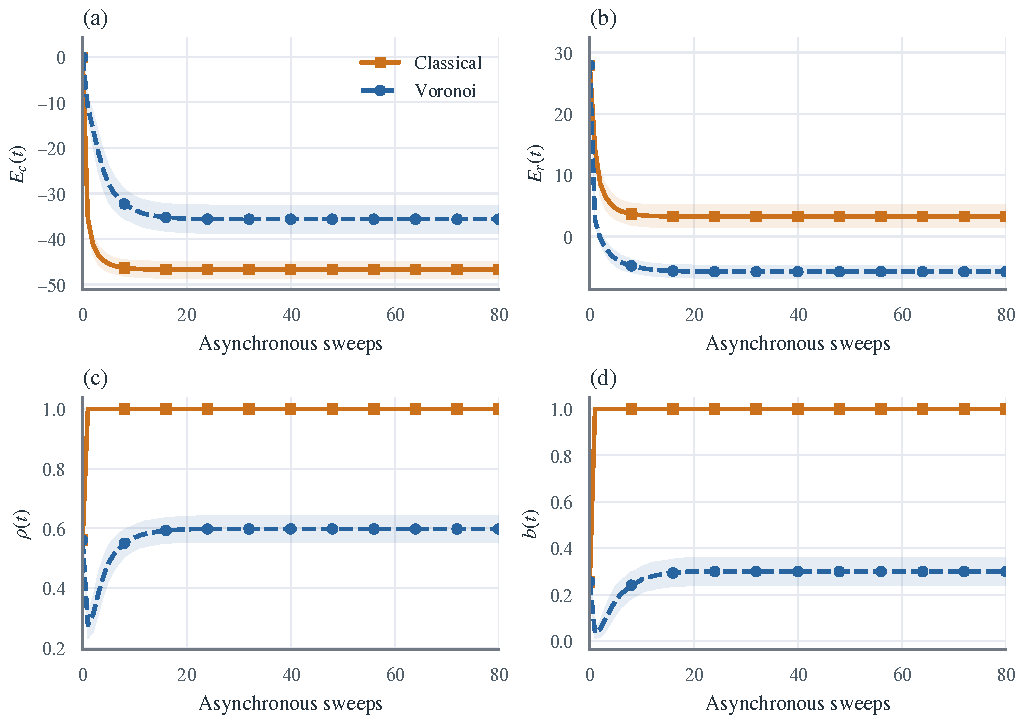
\includegraphics[width=0.86\textwidth]{Figures/saturation_diagnostics.pdf}
    \caption{Geometric and energy diagnostics for 16-QAM under uniform initialization. Solid and dashed curves denote the classical and Voronoi dynamics, respectively; curves show means and shaded bands indicate one standard deviation over $100$ runs. Both energy functionals are evaluated along each trajectory; only $E_c$ for the classical rule and $E_r$ for the Voronoi rule have the corresponding descent guarantee. The Voronoi plateaus are $\rho\approx0.598$ and $b\approx0.299$.}
    \label{fig:exp1_qam_uniform}
\end{figure*}

The numerical snapshot fixes the coordinates and ordering of every alphabet
explicitly in the repository. This prevents equal-radius symbols from being
reordered by platform-dependent floating-point roundoff before random indices
are sampled. Tables and figures are generated from the accompanying
trial-level measurements. A separate hosted replication and its numerical
comparison are also provided. In Experiment~1, $N=100$, and the two update rules share
each of the 100 initial states, weight matrices, and schedules per alphabet
and initialization protocol.

The first experiment isolates the mechanism described in
Section~\ref{sec:bias} and checks, in a controlled numerical setting, the
energy interpretation developed in Section~\ref{sec:voronoi}. The comparison is
between the classical asynchronous rule and the alphabet-dependent Voronoi
activation $\mathcal{D}_{\mathcal{S}}$. The objective is not to test storage
capacity, but to examine whether the local decision rule drives trajectories
toward the amplitude saturation boundary when the state alphabet contains
symbols with nonconstant moduli.

For each finite alphabet $\mathcal{S}$, all symbols are normalized so that
$R_{\max}=1$. The experiment uses PSK as a constant-modulus control case and
the QAM, polar, and hexagonal multi-amplitude families defined in
Section~\ref{sec:prelim} as diagnostic cases. For each Monte Carlo run, a
Hermitian matrix with nonnegative
diagonal is generated in the form
\begin{equation}
    \boldsymbol{W}
    = \alpha\boldsymbol{I}
    + \beta\frac{\boldsymbol{A}_0+\boldsymbol{A}_0^*}{2},
\end{equation}
where the off-diagonal entries of $\boldsymbol{A}_0$ have independent real
and imaginary parts distributed as $\mathcal{N}(0,1/(2N))$, and its diagonal
is zero. We set $\alpha=0$ and $\beta=1$, so the
comparison satisfies the hypothesis $w_{kk}\geq 0$ without introducing positive
self-feedback that could artificially favor radial expansion. Both dynamics are
then run from the same initial state, with the same matrix and the same fair
asynchronous update schedule.

To avoid hiding the effect of initialization, two protocols are reported
separately. The primary protocol samples each component uniformly from the full
alphabet $\mathcal{S}$. A secondary diagnostic protocol samples from the
non-boundary nonzero symbols whenever such symbols exist. The latter setting is
useful for observing radial drift from the interior of a multi-amplitude
constellation, but it is not used as the sole evidence for the saturation
mechanism.

The recorded quantities are the classical Hopfield energy $E_c(t)$, the
inertial energy $E_r(t)$, the normalized squared norm
\begin{equation}
    \rho(t)=\frac{1}{N}\frac{\|\boldsymbol{s}(t)\|^2}{R_{\max}^2},
\end{equation}
where $N$ is the number of neurons introduced in Section~\ref{sec:bias}
and $R_{\max}=\max_{s\in\mathcal{S}}|s|$ is the maximum symbol modulus
from Definition~\ref{def:maximum_modulus} (equal to one after normalization). We also record
the boundary occupation rate, defined as the fraction of neurons located on
the amplitude saturation boundary,
\begin{equation}
    b(t)
    = \frac{1}{N}\sum_{k=1}^{N}
      \mathbf{1}_{\{\,|s_k(t)|=R_{\max}\,\}}.
\end{equation}
In Fig.~\ref{fig:exp1_qam_uniform}, $E_c(t)$ and $E_r(t)$ mean
$E_c(\boldsymbol{s}^{d}(t))$ and $E_r(\boldsymbol{s}^{d}(t))$, respectively,
where $d\in\{c,V\}$ identifies the classical or Voronoi trajectory. Plotting
both functionals for both trajectories provides a common diagnostic: their
gap is exactly $N R_{\max}^2\rho(t)/2$. The classical trajectory's $E_r$
curve therefore measures the same magnitude-corrected objective, without a
general monotonicity guarantee. Its decrease in the displayed mean curve is
an empirical observation, not an additional convergence result.

The experiment also records the number of asynchronous coordinate updates
attempted up to and including the final no-change sweep. Finally, monotonicity violations are counted
for the relevant Lyapunov candidate: $E_c$ for the classical dynamics and
$E_r$ for the $\mathcal{D}_{\mathcal{S}}$ dynamics.

The diagnostic signature of the saturation mechanism is defined for two
types of alphabets distinguished by their moduli. On the one hand, for
constant-modulus alphabets, the classical and Voronoi decisions should coincide
up to tie events, since the quadratic magnitude term is constant over
$\mathcal{S}$. On the other hand, for multi-amplitude alphabets, evidence for the magnitude
saturation bias appears when the classical rule decreases the classical energy
while increasing $\rho(t)$ and $b(t)$ relative to the Voronoi dynamics. By
contrast, evidence for the proposed structural-inertia interpretation appears
when the $\mathcal{D}_{\mathcal{S}}$ dynamics decrease the inertial energy
$E_r(t)$ while avoiding systematic migration toward complete occupation of the
saturation boundary.

The numerical results follow this diagnostic pattern without relying on the
interior initialization protocol. Under uniform initialization, all paired
trajectories converged within the prescribed maximum of $80$ asynchronous
sweeps, and no monotonicity violation was observed for the corresponding
Lyapunov quantity: $E_c$ for the classical rule and $E_r$ for
$\mathcal{D}_{\mathcal{S}}$. Fig.~\ref{fig:exp1_qam_uniform} shows the
representative 16-QAM case. The classical dynamics achieve a lower classical
energy by rapidly moving all components to the outer QAM symbols, as indicated
by $\rho(t)\to 1$ and $b(t)\to 1$. In contrast, the Voronoi dynamics decrease
the inertial energy and settle at a substantially lower norm and boundary
fraction. This illustrates the central point of the paper: the relevant
comparison is not which rule produces the smallest value of $E_c$, but which
energy is aligned with the chosen activation.

The Voronoi plateaus in Fig.~\ref{fig:exp1_qam_uniform} are
$\rho_\infty^V\approx0.598$ and $b_\infty^V\approx0.299$, respectively.
The latter means that, averaged over runs, about $29.9\%$ of the neurons
occupy the four maximum-modulus corner symbols; the remaining neurons occupy
symbols with smaller moduli. The former is the mean squared modulus per
neuron divided by $R_{\max}^2$, not a fraction of boundary neurons or a
recall accuracy. For normalized square 16-QAM, the three squared moduli are
$1/9$, $5/9$, and $1$. If $p_1,p_2,p_3$ denote their occupation fractions,
then $\rho=p_1/9+5p_2/9+p_3$ and $b=p_3$. Hence the two indicators describe
different aspects of the final radial distribution. Their plateau values are
empirical averages determined by the alphabet, weights, initialization, and
update protocol; neither value is a universal target imposed by the inertial
penalty. In particular, the Voronoi rule avoids complete saturation without
requiring the boundary occupation to vanish.

Table~\ref{tab:exp1_uniform_summary} summarizes the same experiment across the
four alphabets. The PSK control behaves as expected: since all symbols have the
same modulus, the two decisions coincide. For QAM, polar, and hexagonal
alphabets, the classical rule reaches full boundary occupation in every run,
whereas $\mathcal{D}_{\mathcal{S}}$ preserves a nontrivial radial distribution.
The superscripts $c$ and $V$ denote the classical and Voronoi dynamics,
respectively. Standard deviations are reported for the
$\mathcal{D}_{\mathcal{S}}$ final values. For the multi-amplitude alphabets, the
corresponding classical final standard deviations are numerically zero because
all runs reached the saturation boundary.
The saturation under the classical rule is not imposed by the code; it follows
from maximizing a homogeneous linear score over a multi-amplitude alphabet,
which tends to select support points on the outer boundary of the constellation.
The secondary inner-initialization protocol produced the same qualitative
ordering and is omitted from the main text for brevity.

\begin{table}[!htbp]
\centering
\caption{Experiment~1 under uniform initialization. Values are Monte Carlo means over $100$ runs.}
\label{tab:exp1_uniform_summary}
\scriptsize
\setlength{\tabcolsep}{2.1pt}
\resizebox{\columnwidth}{!}{%
\begin{tabular}{lcccccc}
\toprule
Alphabet & $\rho(0)$ & $b(0)$ & $\rho_{\infty}^{c}$ & $\rho_{\infty}^{V}$ & $b_{\infty}^{c}$ & $b_{\infty}^{V}$ \\
\midrule
16-PSK & 1.000 & 1.000 & 1.000 & $1.000 \pm 0.000$ & 1.000 & $1.000 \pm 0.000$ \\
16-QAM & 0.561 & 0.255 & 1.000 & $0.598 \pm 0.044$ & 1.000 & $0.299 \pm 0.061$ \\
16-Polar & 0.467 & 0.249 & 1.000 & $0.562 \pm 0.072$ & 1.000 & $0.376 \pm 0.080$ \\
19-Hexagonal & 0.633 & 0.316 & 1.000 & $0.705 \pm 0.045$ & 1.000 & $0.413 \pm 0.060$ \\
\bottomrule
\end{tabular}

}
\end{table}

\subsection{HSV Associative Recall}
\label{sec:exp_hsv_retrieval}

The second experiment tests whether the geometric correction isolated in
Experiment~1 also affects associative recall. We store $P=4$ synthetic HSV
images of size $24\times24$, so that $N=576$, and initialize the network from
corrupted versions of the stored memories. Synthetic HSV patterns are used
instead of an external dataset in order to keep the phase-magnitude encoding
controlled: hue is assigned to phase, saturation to magnitude, and the value
channel is fixed.

For each memory $\mu\in\{1,\ldots,P\}$ and pixel $j$, the HSV representation
has hue $h_j^{\mu}\in[0,1)$, saturation $\sigma_j^{\mu}\in[0,1]$, and value
$V_j^{\mu}$. We fix $V_j^{\mu}=V_0=0.8$ for all pixels. Hence the image
information used by the network is carried by two variables only: hue becomes
phase and saturation becomes modulus. The corresponding continuous complex code
is
\begin{equation}
    \theta_j^{\mu}=2\pi h_j^{\mu}-\pi,
    \qquad
    z_j^{\mu}=R_{\max}\sigma_j^{\mu}e^{\mathbf{i}\theta_j^{\mu}},
\label{eq:hsv_to_complex}
\end{equation}
where $R_{\max}=\max_{s\in\mathcal{S}}|s|$. Given an alphabet
$\mathcal{S}$, the stored symbol is obtained by the static Euclidean quantizer
\begin{equation}
    \xi_j^{\mu}
    =
    Q_{\mathcal{S}}(z_j^{\mu})
    =
    \mathop{\bigwedge}\nolimits_{\preceq}
    \underset{s\in\mathcal{S}}{\arg\min}\, |z_j^{\mu}-s|^2.
\label{eq:hsv_quantization}
\end{equation}
This preprocessing step uses the same Voronoi geometry as
$\mathcal{D}_{\mathcal{S}}$, but it is not a recurrent update.

The inverse map is used only for visualization and red-green-blue (RGB) peak signal-to-noise ratio (PSNR) computation. Given
a recalled complex state $\boldsymbol{x}\in\mathcal{S}^N$, we reconstruct HSV
coordinates by
\begin{equation}
    \widetilde{\sigma}_j
    =
    \min\left\{\frac{|x_j|}{R_{\max}},1\right\},
    \qquad
    \widetilde{V}_j=V_0,
\end{equation}
and, for $x_j\neq0$,
\begin{equation}
    \widetilde{h}_j
    =
    \frac{\operatorname{Arg}(x_j)+\pi}{2\pi}
    \pmod{1}.
\label{eq:complex_to_hsv}
\end{equation}
Here $u\pmod{1}$ denotes the representative of $u$ in $[0,1)$, which is needed
because hue is circular. If $x_j=0$, the hue is arbitrary because
$\widetilde{\sigma}_j=0$ makes it visually irrelevant. All network updates are
nevertheless performed in the complex domain.

After quantization, the memory matrix
$\boldsymbol{X}=[\boldsymbol{\xi}^1,\ldots,\boldsymbol{\xi}^P]\in\mathbb{C}^{N\times P}$
is stored using the projection rule
\begin{equation}
    \boldsymbol{W}
    =
    \boldsymbol{X}(\boldsymbol{X}^*\boldsymbol{X})^{\dagger}\boldsymbol{X}^*,
\label{eq:projection_storage}
\end{equation}
where $\dagger$ denotes the Moore--Penrose pseudoinverse. This matrix is
Hermitian positive semidefinite; hence its diagonal entries are nonnegative,
as required by Theorem~\ref{thm:stability}. For every paired trial, the
classical dynamics and the $\mathcal{D}_{\mathcal{S}}$ dynamics use the same
matrix, corrupted initial state, and asynchronous update schedule.

Two perturbation mechanisms are considered. In symbol perturbations, each
coordinate is replaced, with probability $q$, by a uniformly sampled element of
$\mathcal{S}$. In HSV perturbations, the prequantized image is corrupted by
\begin{align}
    h_j(0)
    &=
    (h_j^{\nu}+\eta_j^{(h)})\pmod{1},
    \\
    \sigma_j(0)
    &=
    \operatorname{clip}
    \bigl(\sigma_j^{\nu}+\eta_j^{(\sigma)},0,1\bigr),
\end{align}
then encoded by \eqref{eq:hsv_to_complex} and quantized by
\eqref{eq:hsv_quantization}. The noise level is the replacement probability
$q$ in the symbol case and the standard deviation of the Gaussian perturbations
in the HSV case. The clipping operation is
$\operatorname{clip}(u,0,1)=\min\{\max\{u,0\},1\}$; it simply keeps saturation
inside the admissible HSV interval.

Retrieval quality is measured after convergence relative to the target memory
$\boldsymbol{\xi}^{\nu}$. Let $d\in\{c,V\}$ denote the selected dynamics,
where $c$ stands for the classical update and $V$ stands for the Voronoi
update. If $\boldsymbol{x}^{d}(\infty)$ is the final state produced by that
dynamics, the symbol error rate (SER) is the normalized Hamming distance
\begin{equation}
    \operatorname{SER}_{d}
    =
    \frac{1}{N}\sum_{j=1}^{N}
    \mathbf{1}_{\{\,x_j^{d}(\infty)\neq \xi_j^{\nu}\,\}},
\end{equation}
and the exact-recovery indicator is
\begin{equation}
    \operatorname{Exact}_{d}
    =
    \mathbf{1}_{\{\,\operatorname{SER}_{d}=0\,\}}.
\end{equation}
We also report the RGB PSNR, obtained after the
inverse HSV map above, and the mean radial error
\begin{equation}
    e_{r,d}
    =
    \frac{1}{N R_{\max}}
    \sum_{j=1}^{N}\bigl||x_j^{d}(\infty)|-|\xi_j^{\nu}|\bigr|.
\end{equation}
Thus $e_{r,d}$ depends on two objects: the stored target
$\boldsymbol{\xi}^{\nu}$ and the final state produced by the chosen dynamics.
It is the most direct diagnostic for the amplitude geometry, because it
measures whether recall preserved the HSV saturation pattern encoded in the
moduli of the complex states. In Table~\ref{tab:exp2_hsv_retrieval}, Exact$_V$
denotes the empirical mean of $\operatorname{Exact}_{V}$ over the paired
Voronoi trials.

The experiment was run on the alphabets 64-PSK, 64-QAM, 64-Polar, and
61-Hexagonal. For the noise experiment, each cell uses 30 paired trials and a
maximum of 80 asynchronous sweeps. The bank contains six patterns generated
with seed 20260901; the noise study stores its first four, with target index
$\nu=1+(r\bmod4)$ for trial $r=0,\ldots,29$. The pseudoinverse uses a relative
singular-value cutoff of $10^{-10}$, and the diagonal of $\boldsymbol{W}$ is
retained. These are corruption and schedule replicates for a fixed memory bank,
not independent draws of memory sets. All trajectories reached a numerical
fixed point, no increase of the corresponding Lyapunov quantity was observed
at a changed coordinate, and the maximum
projection residual $\|\boldsymbol{W}\boldsymbol{X}-\boldsymbol{X}\|/
\|\boldsymbol{X}\|$ was $1.08\times10^{-14}$ in the publication run and
$1.10\times10^{-14}$ in the hosted Colab rerun.

\begin{table}[!t]
\centering
\caption{Experiment~2 under moderate corruption, with $P=4$, $N=576$, and noise level $0.10$. Here, Sym. denotes random symbol replacement and HSV denotes perturbation before quantization.}
\label{tab:exp2_hsv_retrieval}
\scriptsize
\setlength{\tabcolsep}{2.1pt}
\resizebox{\columnwidth}{!}{%
\begin{tabular}{llccccc}
\toprule
Pert. & Alphabet & $\operatorname{SER}_{c}$ & $\operatorname{SER}_{V}$ & $e_{r,c}$ & $e_{r,V}$ & Exact$_V$ \\
\midrule
Sym. & 64-PSK & 0.000 & 0.000 & 0.000 & 0.000 & 1.000 \\
Sym. & 64-QAM & 0.996 & 0.000 & 0.539 & 0.000 & 1.000 \\
Sym. & 64-Polar & 0.996 & 0.200 & 0.551 & 0.025 & 0.700 \\
Sym. & 61-Hex. & 0.997 & 0.000 & 0.535 & 0.000 & 1.000 \\
\midrule
HSV & 64-PSK & 0.178 & 0.178 & 0.000 & 0.000 & 0.600 \\
HSV & 64-QAM & 0.996 & 0.054 & 0.539 & 0.011 & 0.900 \\
HSV & 64-Polar & 0.996 & 0.820 & 0.551 & 0.108 & 0.000 \\
HSV & 61-Hex. & 0.997 & 0.000 & 0.535 & 0.000 & 1.000 \\
\bottomrule
\end{tabular}

}
\end{table}

Table~\ref{tab:exp2_hsv_retrieval} shows the main retrieval behavior at a
moderate noise level. The mean initial SER ranges from $0.094$ to $0.099$ in
the symbol-noise tests and from $0.765$ to $0.935$ in the HSV-noise tests. In
64-PSK, which has constant modulus, the two update rules coincide, confirming
that the proposed correction does not alter the classical decision when radial
information is absent. In contrast, for QAM, polar, and hexagonal alphabets,
the classical rule moves almost all components away from the target memory and
produces radial errors around $0.54$. This happens even though the memories
were stored by projection; the mismatch lies in the classical local decision,
not in the storage rule. The Voronoi dynamics removes this saturation effect.
It gives exact recovery in QAM and hexagonal alphabets under symbol noise,
exact recovery in the hexagonal HSV case, and a 90\% exact recovery rate in the
QAM HSV case. The polar alphabet is more fragile under HSV perturbations, but
even there the Voronoi rule substantially reduces the radial error.

The same radial diagnostic was also evaluated across the tested HSV noise
levels for the 64-QAM case. The classical update remained near a high
radial-error plateau, reflecting a systematic drift toward the outer part of
the constellation. The $\mathcal{D}_{\mathcal{S}}$ update stayed close to zero
radial error under low and moderate perturbations and increased only when the
initial image was strongly displaced. This is precisely the geometric effect
predicted by the inertial energy: the update is no longer rewarded merely for
choosing larger-modulus symbols.

\begin{figure}[!t]
    \centering
    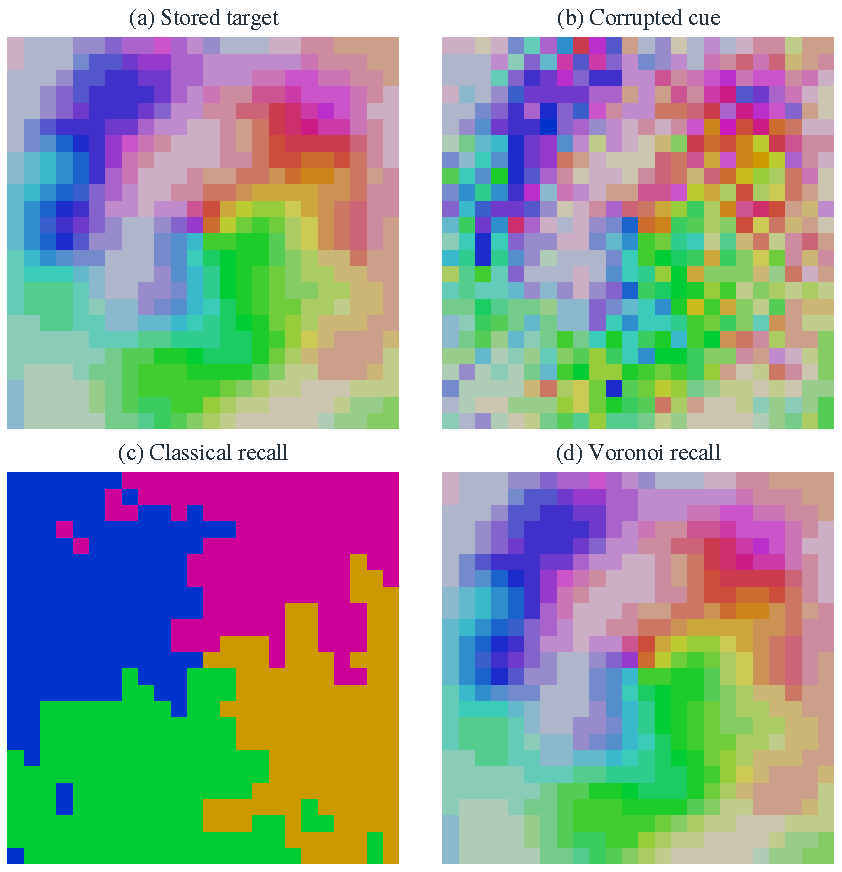
\includegraphics[width=\linewidth]{Figures/hsv_recall.pdf}
    \caption{Illustrative successful 64-QAM recall trial with $P=4$ and HSV noise level $0.10$. This is the successful Voronoi trial with the smallest seed (120044901) in this condition. Aggregate performance includes all 30 trials per condition. The HSV colors encode image content.}
    \label{fig:exp2_visual_panel}
\end{figure}

The visual example in Fig.~\ref{fig:exp2_visual_panel} gives a concrete view of
the same phenomenon. In this trial, the corrupted input has
$\operatorname{SER}(0)=0.804$. The classical update converges to a saturated
image with $\operatorname{SER}_{c}=0.993$ and RGB PSNR $9.10$ dB, whereas
$\mathcal{D}_{\mathcal{S}}$ exactly recovers the stored target with
$\operatorname{SER}_{V}=0$ and zero radial error. The software reports
PSNR $100$ dB as a finite sentinel for zero RGB mean squared error; the
mathematical PSNR is infinite in that case. The classical
recall loses the HSV saturation
structure and produces large saturated regions associated with outer QAM
symbols. The Voronoi recall instead restores the original color pattern. Thus,
the proposed activation is not only a formal modification of the update rule;
in a phase-and-magnitude memory it changes the recovered object in exactly the
degree of freedom targeted by the inertial penalty.

\subsection{Activation Cost}
\label{sec:exp_activation_cost}

The third experiment evaluates the computational cost of applying
$\mathcal{D}_{\mathcal{S}}$. This cost is the main practical question raised
by the proposed activation: for an arbitrary finite alphabet, the nearest
Voronoi center must in principle be found from the set $\mathcal{S}$. The
mathematical decision remains
\begin{equation}
    \mathcal{D}_{\mathcal{S}}(z;s_0)
    \in \Omega_{\mathcal{S}}(z)
    = \underset{s\in\mathcal{S}}{\arg\min}\, |z-s|^2
\label{eq:exp3_exact_activation}
\end{equation}
with the current-state retention and deterministic tie rule defined in
Section~\ref{sec:voronoi}. The experiment compares exact implementations of
this same single-valued decision, including its behavior on shared boundaries.

Four activation procedures are considered. The first is the direct exhaustive
Euclidean search,
\begin{equation}
    \mathcal{D}_{\mathrm{dist}}(z;s_0)
    \in
    \underset{s\in\mathcal{S}}{\arg\min}
    \left[
    (\operatorname{Re}z-\operatorname{Re}s)^2
    +
    (\operatorname{Im}z-\operatorname{Im}s)^2
    \right].
\end{equation}
This method is universal and exact, but it performs a linear scan over the
alphabet. The second is the equivalent exhaustive inertial-score search,
\begin{equation}
    \mathcal{D}_{\mathrm{score}}(z;s_0)
    \in
    \underset{s\in\mathcal{S}}{\arg\max}
    \left[
    \operatorname{Re}(\overline{s}z)-\frac{|s|^2}{2}
    \right],
\label{eq:exp3_inertial_score}
\end{equation}
with $|s|^2/2$ precomputed. This method is also universal and exact, and it is
the computational form most directly aligned with the inertial energy
developed in Section~\ref{sec:voronoi}. The third method stores
$\mathcal{S}$ as points in $\mathbb{R}^2$ and queries an exact nearest-neighbor
KD-tree, a standard spatial data structure for nearest-neighbor search
\cite{bentley1975,friedman1977}. The fourth method uses exact structured
quantizers when the alphabet geometry allows it: angular rounding for PSK,
independent coordinate rounding for square QAM, and a polar-grid search over
the angular sectors and radial levels for polar alphabets. These regular
constellations are common in digital communications, especially PSK and QAM
\cite{proakis2008}. No special structured rule is imposed on the finite
hexagonal patches; for them, the universal methods and the KD-tree are used.
Approximate lookup tables are not included as a primary method because they
introduce an additional grid quantization error and therefore no longer
evaluate \eqref{eq:exp3_exact_activation} exactly.

\begin{table*}[!t]
\centering
\caption{Activation search cores compared in Experiment~3. Arithmetic counts are
expressed in floating-point operations (flops) and exclude tolerance checks
and boundary resolution; a fallback scan can cost $O(|\mathcal{S}|)$.}
\label{tab:exp3_methods}
\scriptsize
\setlength{\tabcolsep}{3.0pt}
\renewcommand{\arraystretch}{1.12}
\begin{tabular}{>{\raggedright\arraybackslash}p{0.16\textwidth}>{\raggedright\arraybackslash}p{0.26\textwidth}>{\raggedright\arraybackslash}p{0.18\textwidth}>{\raggedright\arraybackslash}p{0.24\textwidth}>{\raggedright\arraybackslash}p{0.10\textwidth}}
\toprule
Method & Principle & Query cost & Applicability & Reference \\
\midrule
Euclidean exhaustive &
Compute all squared distances $|z-s|^2$. &
$5|\mathcal{S}|$ flops and $|\mathcal{S}|-1$ comparisons. &
Any finite alphabet; exact reference implementation. &
\cite{aurenhammer2013voronoi} \\
Inertial-score exhaustive &
Maximize $\operatorname{Re}(\overline{s}z)-|s|^2/2$. &
$4|\mathcal{S}|$ flops and $|\mathcal{S}|-1$ comparisons after preprocessing. &
Any finite alphabet; algebraically aligned with $E_r$. &
Sec.~\ref{sec:voronoi} \\
KD-tree &
Store constellation points in $\mathbb{R}^2$ and query nearest neighbors. &
Preprocessing $O(|\mathcal{S}|\log|\mathcal{S}|)$; expected query cost sublinear in low dimension. &
Any finite alphabet; conservative exhaustive fallback on ambiguous ties. &
\cite{bentley1975,friedman1977} \\
Structured quantizer &
Exploit analytic geometry of regular constellations. &
Constant or near-constant cost for PSK and square QAM; small sector/radius search for polar grids. &
Used for PSK, QAM, and polar alphabets; not imposed on finite hexagonal patches. &
\cite{proakis2008} \\
\bottomrule
\end{tabular}
\end{table*}

The experiment uses the same four alphabet families as the previous
experiments with
$|\mathcal{S}|\in\{16,64,256,1024\}$. Two input sample sets are considered. The
first consists of points sampled uniformly from a square containing the
normalized constellation. The second consists of local fields
$z=v_k=(\boldsymbol{W}\boldsymbol{x})_k$ collected from the HSV associative
recall protocol of Experiment~2, using the same projection storage matrix,
corrupted initial states, and Voronoi dynamics. The first sample set measures
generic nearest-neighbor cost in the complex plane, whereas the second measures
the cost on inputs actually produced by the memory dynamics.

Here these four values denote alphabet cardinalities, not neuron counts:
the complex plane has real dimension two and the network used to generate
fields has $N=576$ and $P=4$ throughout. Its memories are the first four
patterns of the same six-pattern bank used in Experiment~2. Uniform fields
are drawn from $[-1.25R_{\max},1.25R_{\max}]^2$; network fields are sampled
initially and after up to three Voronoi sweeps following HSV perturbations
of standard deviation $0.10$. Network queries carry the current symbol of
the corresponding neuron. Uniform queries receive a uniformly sampled
current symbol. Every method receives the same fields and current symbols.

For each method, alphabet, and input sample set, the recorded quantities are:
agreement with the exhaustive Euclidean search, average query time,
preprocessing time, estimated arithmetic count, number of
comparisons, and the ratio between activation cost and dense local-field update
cost. Agreement is the fraction of queries for which a method returns the same
symbol as the exhaustive Euclidean reference. The average query time is
reported in microseconds per local field, preprocessing time is measured once
per alphabet. For one query, the exhaustive Euclidean
rule uses approximately $5|\mathcal{S}|$
floating-point operations and $|\mathcal{S}|-1$ comparisons, while the
inertial-score rule uses approximately $4|\mathcal{S}|$ floating-point
operations and $|\mathcal{S}|-1$ comparisons after precomputing
$|s|^2/2$. With incremental asynchronous updates for a dense matrix
$\boldsymbol{W}\in\mathbb{C}^{N\times N}$, one full sweep costs approximately
$8N^2$ floating-point operations for maintaining the local field. Thus, the
activation-to-field cost ratios for the two exhaustive exact searches are
\begin{equation}
    \chi_{\mathrm{dist}}
    =
    \frac{5|\mathcal{S}|}{8N},
    \qquad
    \chi_{\mathrm{score}}
    =
    \frac{4|\mathcal{S}|}{8N}.
\label{eq:activation_field_ratio}
\end{equation}
These ratios separate the mathematical cost of the proposed activation from
the cost of the recurrent Hopfield computation itself.

The benchmark uses one BLAS thread, one KD-tree worker, $20{,}000$ queries
per input sample set, a warm-up, and five timing repetitions. Method order
rotates between repetitions. The measured operation includes current-state
retention and numerical tie resolution; preprocessing and field generation
are excluded. KD-tree and structured searches detect competing nearest
candidates and fall back to the ordered exhaustive rule on ambiguous
boundaries. Thus their fast-path cost is not a worst-case bound.
Correctness is checked before timing, on the sampled fields and separately
on nearest-neighbor midpoints and the origin, both with and without a current
symbol. All tested decisions agree with the exhaustive reference.

\begin{figure*}[!t]
\centering
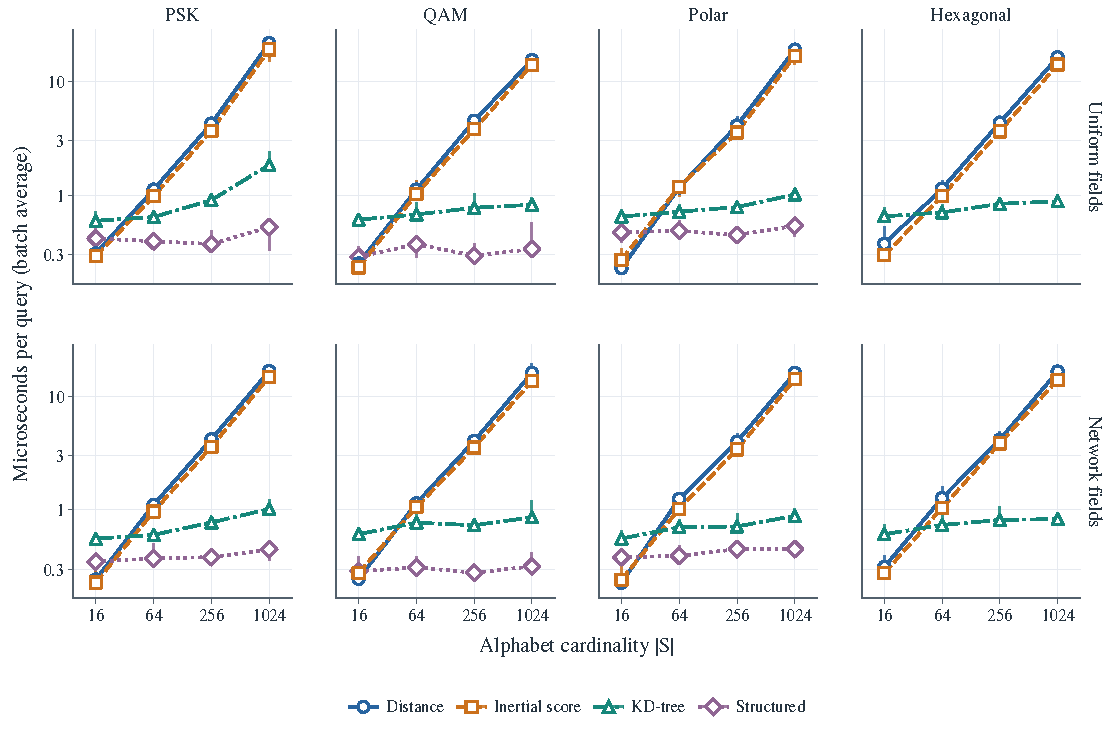
\includegraphics[width=\textwidth]{Figures/activation_scaling.pdf}
\caption{Activation cost across alphabet cardinalities
$|\mathcal{S}|\in\{16,64,256,1024\}$. Columns show alphabet families; rows
show uniform and network-generated fields. Markers are medians of five
repetitions, and vertical bars show their full range. Each repetition times
a batch of $20{,}000$ queries; the ordinate is batch time divided by query
count. Both axes are logarithmic. Colors, markers, and line patterns identify
methods. All methods include conservative tie handling. The network has
$N=576$ throughout; the figure does not vary the number of neurons.}
\label{fig:activation_scaling}
\end{figure*}

Figure~\ref{fig:activation_scaling} reports the complete cardinality sweep.
The relative cost depends
on alphabet size and on the field distribution: fixed overhead matters for
small alphabets, whereas exhaustive scans must evaluate all symbols as the
alphabet grows. Structured geometry and spatial search can reduce that work,
but their benefit must be measured with the same boundary convention.
The inertial-score expression saves arithmetic in the search core; this does
not by itself establish a wall-clock advantage once array allocation,
comparison, and tie handling are included.
In the publication run, at cardinality 16, exhaustive search is faster than KD-tree search for both
input sets in all four families. At cardinality 1024, the structured method
is fastest for PSK, QAM, and polar alphabets, while KD-tree search is fastest
among the tested methods for the hexagonal patches. Thus the choice of
implementation should depend on alphabet size and structure rather than on
the asymptotic search cost alone.

These measurements concern vectorized batch throughput on the recorded
machine. They do not establish single-call latency or an equal acceleration
of the complete network, whose local fields must also be maintained. The
analytical ratios in \eqref{eq:activation_field_ratio} describe that separate
cost. A full rerun of the source code in hosted Google Colab preserved
the method rankings at cardinalities 16 and 1024 stated above, although
individual median times were approximately 0.63--4.98 times their
publication-host values. The publication and rerun timing datasets and their
environments are archived separately. None of the timing comparisons
changes the convergence argument.

\subsection{Code and Data Availability}
The Python implementations, trial-level measurements, ordered alphabet
coordinates, coordinate-level energy audits, figure generators, and four
Google Colab notebooks are publicly available in the companion
repository~\cite{castro2026complexsoftware}:
\url{https://github.com/Fideliszan/complex-valued-voronoi-hopfield}.
Version~1.0.2 identifies the computational companion to this manuscript.
The complete source package distributed with the manuscript also contains
the companion. The notebooks download the public source and run the same
experimental protocols without requiring GitHub credentials.
Reported benchmark times describe the recorded machine; fresh runs record
their own environment and timings.

An additional full execution of the computational protocols on Google Colab
reproduced all saturation trajectories and all recall outcomes, symbol
errors, and stopping counts. Differences in recall energies were below
$4\times10^{-13}$. The coordinate-energy checks passed, and all tested
activation decisions agreed with exhaustive search. The numerical inputs to the five manuscript figures were also checked
there. The current figure typography was regenerated locally from those
validated inputs. The companion preserves the raw
hosted measurements, numerical environments, and comparison checks
separately from the publication-host timing data.

\section{Concluding Remarks} 
\label{sec:conclusion}

In this paper, we investigated CV-HNNs
whose states belong to finite alphabets in the complex plane. The starting
point was the observation that the classical inner-product activation is well
suited to phase-only or constant-modulus alphabets, but it may be geometrically
biased when the admissible symbols have different magnitudes. Precisely, the
classical score can favor outer symbols because the candidate magnitude enters
the decision multiplicatively. We referred to this effect as the magnitude
saturation bias.

To overcome this limitation, we introduced the alphabet-dependent activation
$\mathcal{D}_{\mathcal{S}}$, defined by the Voronoi projection induced by the
chosen constellation. This formulation makes the geometry of the state space
part of the model itself and applies, without changing the basic update
principle, to PSK, QAM, polar, hexagonal, and irregular finite alphabets. We
also showed that this activation is naturally associated with an inertial
energy. The local Voronoi decision is equivalent to maximizing an
inner-product score penalized by the candidate squared modulus, which explains
why the Lyapunov functional involves $\boldsymbol{W}-\boldsymbol{I}$. Under
Hermitian weights with nonnegative diagonal entries, fair asynchronous updates,
and conservative deterministic tie handling, this energy decreases at every
non-stationary transition. Consequently, the proposed dynamics reaches a fixed
point after finitely many such transitions.

The computational experiments complement the theoretical analysis. First, the
geometric diagnostic confirms that the classical update drives multi-amplitude
states toward the saturation boundary, whereas
$\mathcal{D}_{\mathcal{S}}$ preserves a nontrivial radial distribution. Second,
the HSV associative-memory experiment shows that this radial effect is visible
in a recall task in which hue and saturation are encoded as phase and
magnitude. Third, the cost experiment indicates that exact implementations of
the Voronoi activation need not rely on a naive exhaustive scan: KD-tree search
and structured quantizers provide substantial accelerations whenever the
constellation geometry permits them.

Finally, we emphasize the scope of the results. The convergence theorem is a
fixed-point result for the proposed asynchronous dynamics; it does not
constitute a storage-capacity theorem, a guarantee of perfect recall for
arbitrary memories, or a proof that spurious attractors are absent. Likewise,
the reported running times are implementation-dependent and should be read
together with the floating-point operation count. Future work should investigate capacity, basin
geometry, and spurious fixed points under different alphabets and learning
rules. It should also consider larger constellations, optimized implementations
of the activation, and extensions of the inertial-energy viewpoint to
hypercomplex Hopfield models.


\bibliographystyle{IEEEtran}
\bibliography{references}

\end{document}
